\documentclass[12pt]{amsart}
\usepackage[T1]{fontenc}
\usepackage{amsmath}
\usepackage{amssymb}
\usepackage{tikz}
\usepackage{tikz-cd}

\begin{document}

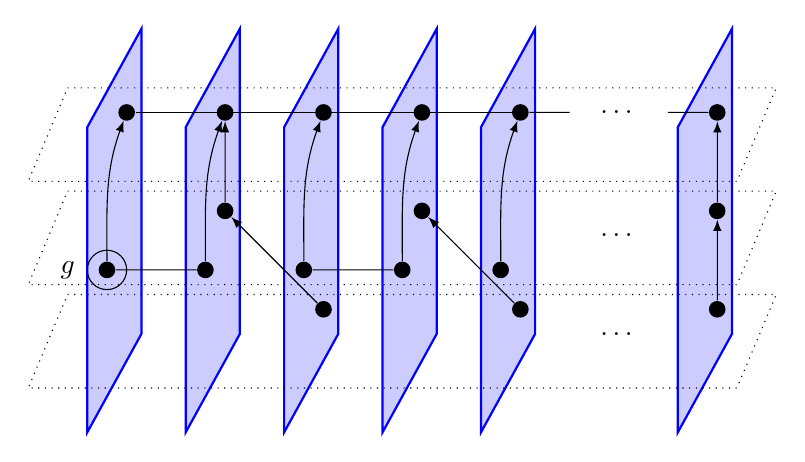
\begin{tikzpicture}[
    scale=1.25,
    dot/.style={circle,fill=black,minimum size=6pt,inner sep=0}
]

\foreach \x in {0,...,4,6} {
    \draw[blue,thick,fill=blue!20] (\x - 0.4, -1.25) -- (\x - 0.4, 1.85) -- (\x + 0.15, 2.85) -- (\x + 0.15, -0.25) --cycle;
}

\foreach \y in {2.05, 1, -0.05} {
    \draw[dotted] (-0.6, \y + 0.2) -- (6.6, \y + 0.2) -- (6.2, \y - 0.75) -- (-1, \y - 0.75) -- cycle;
}

\node (C2) [dot] at (-0.2, 0.4) {};
\node (D2) [dot] at (0.8, 0.4) {};
\node (E2) [dot] at (1, 1) {};
\node (F3) [dot] at (2, 0) {};
\node (G2) [dot] at (1.8, 0.4) {};
\node (H2) [dot] at (2.8, 0.4) {};
\node (I2) [dot] at (3, 1) {};
\node (J3) [dot] at (4, 0) {};
\node (K2) [dot] at (3.8, 0.4) {};
\node at (5, 0.75) {$\dots$};
\node at (5, -0.25) {$\dots$};
\node (LIM2) [dot] at (6, 1) {};
\node (LIM3) [dot] at (6, 0) {};

\node (A1) [dot] at (0, 2) {};
\node (B1) [dot] at (1, 2) {};
\node (C1) [dot] at (2, 2) {};
\node (D1) [dot] at (3, 2) {};
\node (E1) [dot] at (4, 2) {};
\node at (5, 2) {$\dots$};
\node (LIM1) [dot] at (6, 2) {};

\draw (C2) -- (D2);
\draw[-latex] (F3) -- (E2);
\draw[-latex] (J3) -- (I2);
\draw (G2) -- (H2);

\draw (A1) -- (E1);
\draw (E1) -- (4.5, 2) {};
\draw (5.5, 2) -- (LIM1) {};

\draw[-latex] (E2) -- (B1);

\draw[-latex] (C2) to[out=90, in=250] (A1);
\draw[-latex] (D2) to[out=90, in=250] (B1);
\draw[-latex] (G2) to[out=90, in=250] (C1);
\draw[-latex] (H2) to[out=90, in=250] (D1);
\draw[-latex] (K2) to[out=90, in=250] (E1);
\draw[-latex] (LIM2) to (LIM1);
\draw[-latex] (LIM3) to (LIM2);

\draw (C2) circle[radius=0.2];
\node at (-0.6, 0.4) {$g$};

\end{tikzpicture}

\end{document}